\documentclass[11pt]{article}    
\usepackage[a4paper,left=1in,right=1in,top=1in,bottom=1in]{geometry} 

\usepackage[english]{babel}
\usepackage[T1]{fontenc} 
\usepackage[utf8]{inputenc}
\usepackage{seqsplit}

\renewcommand{\familydefault}{\sfdefault} 
\usepackage{setspace}  \singlespacing  
\usepackage{graphicx}        
\usepackage[absolute]{textpos}
\usepackage{xcolor}
\usepackage{fontawesome5}
\usepackage{multirow}
\usepackage{hyperref}
\hypersetup{
    colorlinks,
    linkcolor={red!50!black},
    citecolor={blue!50!black},
    urlcolor={blue}
}

% Additional packages for the content
\usepackage{float}
\usepackage{subfig,wrapfig}
\usepackage{amsmath,amsfonts,amsthm,amssymb}
\usepackage{fancyhdr,fancybox,color}
\usepackage{enumerate}
\usepackage[amssymb]{SIunits}
\definecolor{MyBlue}{rgb}{0,0.3,0.6}

\usepackage{tcolorbox}
\definecolor{mgray}{gray}{0.85}
\definecolor{mpurple}{HTML}{68236D}

\usepackage[all]{hypcap}
\usepackage{csquotes}
\usepackage[url=false,
backend=bibtex,
style=authoryear-comp,
doi=true,
isbn=true,
backref=false,
dashed=false,
maxcitenames=2,
maxbibnames=99,
natbib=true]{biblatex}
\DeclareNameAlias{author}{family-given}
\renewbibmacro{in:}{}
\addbibresource{../_logosAndRef/references.bib}
\nonfrenchspacing

% Configurable separation between header and body
\newlength{\headertobodysep}
\setlength{\headertobodysep}{1cm}

% Header with logos and contact information
\begin{document}
\thispagestyle{empty}

% Lean header with aligned elements
\textblockorigin{0pt}{0pt}

% Durham logo on the left
\begin{textblock*}{5cm}(0.5cm,1cm)
    
\includegraphics[height=2cm]{../_logosAndRef/Durham-University.pdf}
\end{textblock*}

% Contact information in the center - vertically centered with logos
\begin{textblock*}{9cm}(6cm,1.5cm)
    \centering
    {\large \textbf{Drops and bubbles spreading | CoMPhy Lab}}\\[0.2em]
    Department of Physics, Durham University\\[0.3em]
    \href{https://comphy-lab.org}{comphy-lab.org}
\end{textblock*}

% CoMPhy logo aligned with right margin
\begin{textblock*}{5cm}(15.5cm,1cm) % exactly 1 cm away from the right edge
    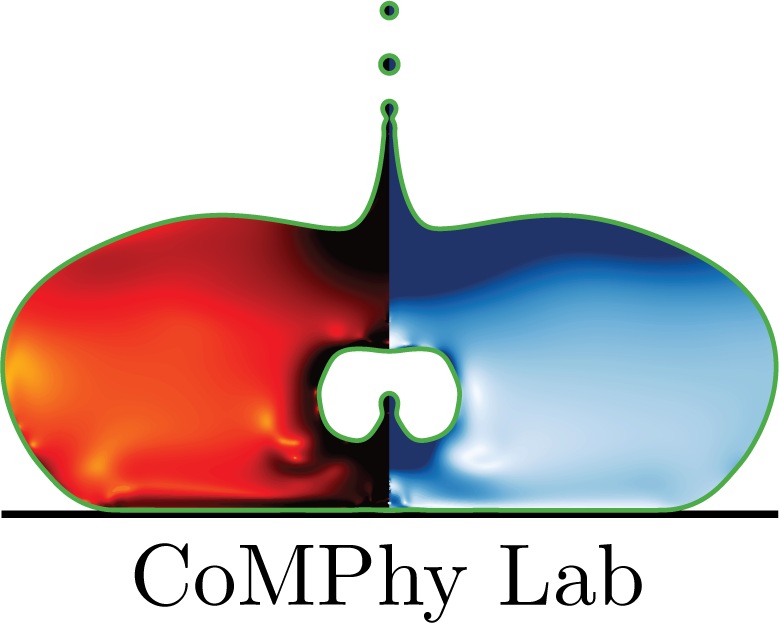
\includegraphics[height=2cm]{../_logosAndRef/CoMPhy-Lab.png}
\end{textblock*}

% Reset to normal text flow after header
\vspace*{\headertobodysep}

\begin{center}
    \begin{LARGE}
     Drops and bubbles spreading on lubricant infused surfaces
    \end{LARGE}
\end{center}

\noindent Watch a water drop dance on a non-stick pan, or an air bubble slide along a submerged leaf -- these everyday phenomena hide rich physics at the intersection of surface tension, viscosity, and topology.

\begin{tcolorbox}[colback=mgray,colframe=mpurple,title=TL;DR]
    Liquid-infused surfaces (LIS) enable unprecedented control over fluid spreading, crucial for self-cleaning materials and microfluidics. This project investigates how drops and bubbles spread on lubricant-laden substrates through high-resolution numerical simulations. Using Basilisk's adaptive VOF solver, you'll capture the cascade of capillary waves triggered when fluids contact LIS, map spreading regimes and reveal how wave convergence entrains secondary droplets. Working with experimentalists at TU Delft and Univ. Twente, you'll develop scaling laws bridging microscopic contact lines to macroscopic spreading, advancing both fundamental understanding and applications in anti-fouling coatings and heat transfer.
\end{tcolorbox}

\section*{Description}

Liquid-infused surfaces (LIS) represent a breakthrough in controlling how fluids spread on solids, with applications from self-cleaning materials to drag reduction. 
When drops or bubbles contact these lubricant-laden substrates, the topology change at the three-phase contact line triggers cascading capillary waves that reshape the interface (fig.~\ref{Figure::Typical}). This project investigates the fundamental spreading dynamics of liquid drops and air bubbles on LIS through direct numerical simulation. You will use volume-of-fluid methods to resolve the multi-scale physics -- from microscopic contact lines to macroscopic wave propagation -- and map how viscosity ratios, surface tensions, and geometric parameters control spreading behaviour. The work will reveal how capillary waves converge to entrain secondary droplets/bubbles, identify the competing timescales (viscous, inertial, capillary) governing the dynamics, and establish scaling laws for spreading rates. These insights will guide the design of LIS for applications in microfluidics, heat transfer, and anti-fouling coatings.

\begin{figure}
	\begin{center}
		\includegraphics[width=0.95\textwidth]{BubbleOnLIS.pdf}
		\caption{A typical scenario of an air bubble in water spreading on liquid infused surfaces (LIS). In each snapshot, left-hand side contains information about the velocity field magnitude normalized with the inertio-capillary velocity and the right-hand side shows viscous dissipation function ($\varepsilon_\eta = 2\eta\left(\boldsymbol{\mathcal{D}:\mathcal{D}}\right)$). The latter is plotted on a $\log$ scale to identify regions of high viscous dissipation. Also see the video of this process at: \href{https://www.youtube.com/watch?v=crRoP9udk9M}{https://www.youtube.com/watch?v=crRoP9udk9M}.}
		\label{Figure::Typical}
\end{center}
\end{figure}

\section*{Deep dive}

The main objectives of this study are:

\begin{enumerate}
	\item To investigate the spreading behavior of liquid drops and air bubbles on LIS under different conditions, such as liquid and geometric properties (see figure~\ref{Figure::Typical}). 
	\item To understand the underlying mechanisms that govern the spreading behavior of liquid drops and air bubbles on LIS. 
	\item To identify and explore the different timescales relevant for this process (see the introduction of \citet{VatsalThesis}).
\end{enumerate}

\noindent \textbf{Problem formulation:} The spreading process involves three immiscible phases (drop/bubble, ambient fluid, lubricant) with distinct densities $\rho_i$ and viscosities $\eta_i$. The dynamics are governed by the incompressible Navier-Stokes equations with surface tension forces $\gamma_{ij}$ at each interface. Key dimensionless groups include the Ohnesorge number $Oh_i = \eta_i/\sqrt{\rho_o\gamma_{ow}R}$ comparing viscous to inertio-capillary effects, density and ratio of interfacial energies. 

\noindent \textbf{Numerical setup:} We will employ the volume-of-fluid (VOF) method with geometric reconstruction in \href{https://github.com/comphy-lab/Bubble-at-Lubis}{Basilisk C} to track the evolving interfaces. The adaptive mesh refinement targets the contact line region and capillary waves, with maximum refinement. Time integration also uses an adaptive scheme.

\noindent \textbf{Validation and uncertainty:} Simulations will be validated against: (i) experimental high-speed imaging data from collaborators at TU Delft/Univ. Twente, (ii) analytical solutions for small-amplitude capillary waves, (iii) grid convergence studies monitoring integrated kinetic energy and enstrophy. The viscous dissipation function $\varepsilon_\eta = 2\eta\left(\boldsymbol{\mathcal{D}:\mathcal{D}}\right)$ will quantify energy loss pathways.

\section*{What will you do and what will you learn?}
In the Physics of Fluids group, we are looking for enthusiastic students to work on this topic.
\begin{enumerate}
\itemsep0em
\item You will learn about fundamental fluid dynamics.
\item You will get hands-on experience with Computational Fluid Dynamics (CFD).
\item You will learn how to do basic and advanced data analysis.
\item You will learn modeling of complex multiphase systems contact lines. 
\item You will learn how to document and publish read-to-use codes and share them with the community, similar to \citet{basiliskVatsal, basiliskVatsalDropFilm, basiliskVatsalViscousBouncing}. 
\item As a part of the \href{https://comphy-lab.org}{CoMPhy lab}, you will learn and adapt open-source coding principles. 
\item You will learn how to collaborate with a diverse group of researchers, specifically with other numericists, experimentalists and theoreticians.
\end{enumerate}

If you have any questions, feel free to contact us \href{mailto:vatsal.sanjay@comphy-lab.org}{vatsal.sanjay@comphy-lab.org}/\\\href{mailto:vatsal.sanjay@durham.ac.uk}{vatsal.sanjay@durham.ac.uk} or drop by Ph255 (Rochester building) at the Department of Physics at Durham University.

\begin{center}
\begin{tabular}{|l|l|l|}
\hline \textbf{Collaborators} & \textbf{E-mail} & \textbf{Based at} \\
\hline \multirow{2}{*}{Dr. Vatsal Sanjay} & \href{mailto:vatsal.sanjay@comphy-lab.org}{vatsal.sanjay@comphy-lab.org} & \multirow{2}{*}{Ph255 (Rochester building)} \\
& \href{mailto:vatsal.sanjay@durham.ac.uk}{vatsal.sanjay@durham.ac.uk} & \\
\hline Aman Bhargava M.Sc. & \href{mailto:a.s.bhargava@utwente.nl}{a.s.bhargava@utwente.nl} & Univ. Twente \\
\hline Dr. Alexandros Oratis   & \href{mailto:a.t.oratis@tudelft.nl}{a.t.oratis@tudelft.nl}& TU Delft \\
\hline Prof. Dr. Detlef Lohse F.R.S. & \href{mailto:d.lohse@utwente.nl}{d.lohse@utwente.nl} & Univ. Twente  \\
\hline
\end{tabular}
\end{center}

\vspace{1em}
\noindent\textit{Last updated: \today}

\printbibliography

\end{document}